\section{Background}

ND is a logical proof system that reflects mathematical and everyday reasoning under assumptions~\cite{nd-mancosu}. It emerged in 1934 with Gentzen and Jaśkowski's work, gaining widespread acceptance by the 1960s~\cite{Pelletier1999-FRAABH}. Using ND, an important goal is to verify whether a formula \(\varphi\) is a semantic consequence of a set of formulas \(\Gamma\), written \(\Gamma \vdash \varphi\). This means that whenever all formulas in \(\Gamma\) hold, \(\varphi\) must also hold because it logically follows from \(\Gamma\) \cite{gouveia_lgica1, gouveia_lgica2}. There are many ways to represent these proofs. The two main styles that exist are the Gentzen style, which organizes the proof in a tree-shaped structure, and the Fitch style, which uses a linear structure with deeper indentation levels to represent assumptions or intermediate steps in the proof. Our article focuses on the first one. 

Gentzen style uses tree-shaped structures, also known as deduction trees. These structures represent proofs and are built by starting with individual trees, which are formulas, and successively applying rules of inference to generate new and more complex trees. The formula at the root is the conclusion of the proof, and formulas at the leaves are called hypotheses and are generally associated with marks. In this article, we use numbers to denote such marks. Marks are used to identify distinct assumptions and to indicate when they are discharged (closed). A hypothesis is considered discharged if its mark is referenced by a rule. Rules are represented using fractions (a horizontal line), where hypotheses appear above the line and the rule’s conclusion appears below. The rule’s name and the marks for the hypotheses are normally placed on the right-hand side of the fraction. There are two main groups of rules for each logical connective: introduction (\(I\)), which constructs more complex formulas from simpler ones, and elimination (\(E\)), which extracts information from complex formulas. Additionally, a special rule, known as absurdity (\(\bot\)), allows deriving any conclusion from a contradiction. Each rule has its own characteristics, and some can only be applied under specific circumstances, called side conditions. For simplicity, we do not discuss these here, but they are included in our algorithm. Figure \ref{fig:nd-rules}, list all the rules considered in our implementation. Greek letters represent generic formulas. The symbols \( \mathcal{D} \) represent subtrees within branches, while \( m \) and \( n \) denote marks. The notation \(\displaystyle \left[ \varphi \right]^a_{\substack{b}}\) indicates the substitution (or mapping) of terms from \( a \) to \( b \), and \(\displaystyle [\varphi]^m\) represents which assumptions can be used in each branch by the rule.

\begin{figure}
    \centering
    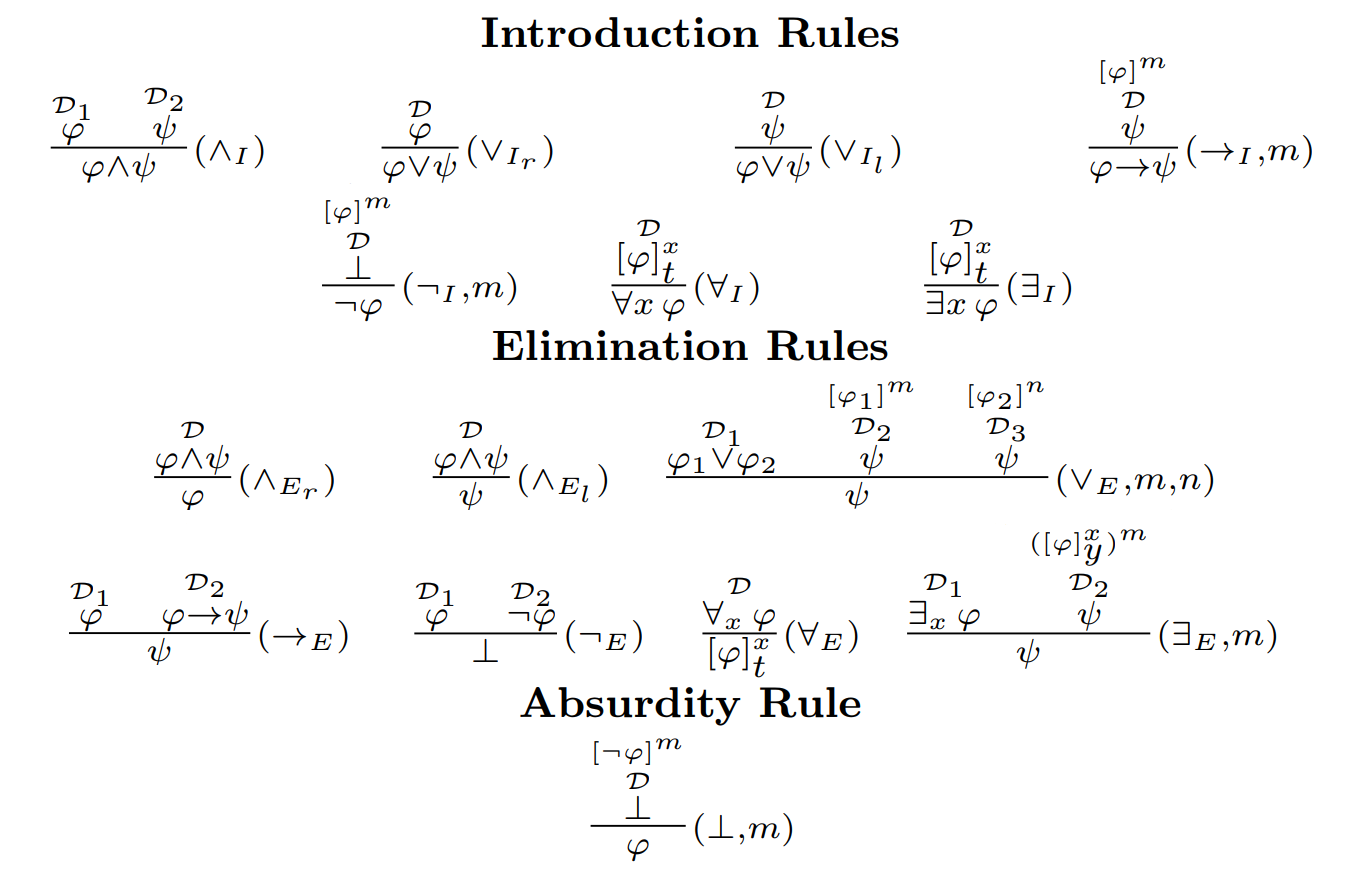
\includegraphics[width=1\linewidth]{resources/rules.png}
    \caption{List of rules for both PL and FOL}
    \label{fig:nd-rules}
\end{figure}

These proofs can be constructed either bottom-up, from the conclusion to the hypotheses, or top-down, from the hypotheses to the conclusion. Figure \ref{tab:proof-tree} shows an example of a proof, where the goal is to prove: \( \{\neg (\varphi \lor \psi)\} \vdash \neg \psi \).

\begin{figure}
    \centering
    \[
    \frac{\displaystyle \frac{
    \displaystyle \neg (\varphi \lor \psi)^1 \quad \displaystyle \frac{\psi^2}{(\varphi \lor \psi) \strut} \quad (\lor_{I_l}) \strut}
    {\displaystyle \bot \strut} \quad (\displaystyle \neg_E)\strut} {\displaystyle \neg \psi \strut} \quad (\neg_I, 2)
    \]
    \caption{Tree proving \( \{\neg (\varphi \lor \psi)\} \vdash \neg \psi \).}
    \label{tab:proof-tree}
\end{figure}


\begin{definition}[Well-Formed Tree Proof]
A tree proof is well-formed if and only if it is finite and applies the inference rules correctly.
\end{definition}

\begin{definition}[Tree Proof Correctness]
Given a tree proof and a problem \(\Gamma \vdash \phi\), we say that the tree solves the problem if and only if it is well-formed and both of the following conditions hold:
\begin{enumerate}
    \item The root of the tree is \(\phi\).
    \item Every open hypothesis in the tree is contained in \(\Gamma\).
\end{enumerate}
\end{definition}